% WACV 2027 Vision4Neuro CAMERA-READY (accepted 2026-10-29). Changes requested by the Program Chairs: claims scoped to
% frozen same-goal transfer AND a moved-goal test; pose belief and evaluation policy clarified with loop-rate reporting;
% replay (E3), predicted-cortex and alignment studies moved to the supplement; retitled. All units are percentage points (pp).
% New numbers: data/audit/v4n_camera_ready_20261031 (PROTOCOL.json written before any new outcome; analysis.json, bc_heldout.json).
\documentclass[10pt,twocolumn,letterpaper]{article}
\usepackage[workshop]{wacv}
%% This file contains a number of tweaks that are typically applied to the main document.
%% They are not enabled by default, but can be enabled by uncommenting the relevant lines.


%%
%% Official support for 2-column teaser figure
%%
% \usepackage{cuted} % strip environment unused; it left page 8's right column empty after the float page

%%
%% For auto-referencing of figures (see fig/teaser.tex and \label{} therein) 
%%
\usepackage{currfile} %< for \currfilebase macro

%%
%% caption and (global) spacing overrides
%%
\usepackage{caption} %< for "\captionof" commands (teaser)
% \setlength{\abovecaptionskip}{.5em} % space above caption
% \setlength{\belowcaptionskip}{1em} % space below caption

%%
%% Inline annotations; for predefined colors, refer to "dvipsnames" in the xcolor package:
%% https://tinyurl.com/overleaf-colors
%%
\newcommand{\red}[1]{{\color{red}#1}}
\newcommand{\todo}[1]{{\color{red}#1}}
\newcommand{\TODO}[1]{\textbf{\color{red}[TODO: #1]}}
%%
%% Disable for camera ready / submission by uncommenting these lines:
%%
% \renewcommand{\TODO}[1]{}
% \renewcommand{\todo}[1]{#1}

%%
%% Work harder in optimizing text layout. Typically shrinks text by 1/6 of page, enable
%% it at the very end of the writing process, when you are just above the page limit.
%%
% \usepackage{microtype}

%%
%% Fine-tune paragraph spacing.
%%
% \renewcommand{\paragraph}[1]{\vspace{.5em}\noindent\textbf{#1.}}

%%
%% Globally adjusts space between figure and caption.
%%
% \setlength{\abovecaptionskip}{.5em}

%%
%% Allows "the use of \paper to refer to the project name"
%% with automatic management of space at the end of the word.
%%
% \usepackage{xspace}
% \newcommand{\paper}{ProjectName\xspace}

%%
%% Commonly used math definitions.
%%
% \DeclareMathOperator*{\argmin}{arg\,min}
% \DeclareMathOperator*{\argmax}{arg\,max}

%%
%% Tighten underline.
%%
% \usepackage{soul}
% \setuldepth{foobar}

%%
%% Reconfigure paragraph (tweaks spacing)
%%

\usepackage{booktabs,tabularx,amsmath,amssymb,graphicx,placeins}
\definecolor{wacvblue}{rgb}{0.21,0.49,0.74}
\usepackage[pagebackref,breaklinks,colorlinks,allcolors=wacvblue]{hyperref}
\def\wacvPaperID{20}
\def\confName{WACV}
\def\confYear{2027}
% generated by scripts/v4n_camera_numbers_claude.py; do not edit
\newcommand{\HLrevisit}{8.2}
\newcommand{\HLrevisitlo}{6.0}
\newcommand{\HLrevisithi}{10.5}
\newcommand{\HLtrap}{8.7}
\newcommand{\Ftrap}{95\%}
\newcommand{\Bclean}{100\%}
\newcommand{\Bcleanp}{0.996}
\newcommand{\Bdim}{44\%}
\newcommand{\SAhuman}{43}
\newcommand{\GRhuman}{32}
\newcommand{\BCrat}{56\%}
\newcommand{\BChuman}{66\%}
\newcommand{\BClegalrat}{32\%}
\newcommand{\BClegalhuman}{31\%}
\newcommand{\BCinforat}{0.25}
\newcommand{\BCinfohuman}{0.55}
\newcommand{\NatHum}{3.8}
\newcommand{\NatRat}{14.4}
\newcommand{\LoopInt}{1.7}
\newcommand{\LoopIntlo}{0.6}
\newcommand{\LoopInthi}{2.9}
\newcommand{\LoopSlope}{0.94}
\newcommand{\NoiseTrapH}{46}
\newcommand{\CleanTrapH}{55}
\newcommand{\NoiseTrapL}{58}
\newcommand{\CleanTrapL}{64}
\newcommand{\PMvLegal}{2.0}
\newcommand{\PMvLegallo}{0.3}
\newcommand{\PMvLegalhi}{3.6}
\newcommand{\PMvLegalp}{0.043}
\newcommand{\PMvScratch}{3.8}
\newcommand{\PMvScratchlo}{2.5}
\newcommand{\PMvScratchhi}{5.1}
\newcommand{\PMvScratchp}{8.4\times10^{-6}}
\newcommand{\PMvRat}{-1.3}
\newcommand{\PMvRatlo}{-2.4}
\newcommand{\PMvRathi}{-0.1}
\newcommand{\PMvRatp}{0.043}
\newcommand{\PGreedy}{7.3}
\newcommand{\PGreedylo}{4.6}
\newcommand{\PGreedyhi}{9.9}
\newcommand{\PGreedyp}{1.5\times10^{-5}}
\newcommand{\MVratbc}{4.4}
\newcommand{\MVratlegaluniform}{5.6}
\newcommand{\MVratsham}{5.2}
\newcommand{\MVhumanbc}{9.4}
\newcommand{\MVhumanlegaluniform}{7.5}
\newcommand{\MVcoldppo}{5.7}
\newcommand{\MVoldgoalH}{40\%}
\newcommand{\MVoldgoalL}{30\%}
\newcommand{\MVoldgoalD}{10.1}
\newcommand{\MVtrapD}{6.6}

% Claims that depend on the moved-goal, greedy and learning outcomes (written after the registered analyses completed).
\newcommand{\MGabstract}{When the goal moves, frozen human-choice agents still loop less but also head back to the old goal: their gain shrinks to \PMvLegal\ pp.}
\newcommand{\MGresults}{All frozen agents now succeed below a uniform policy (\MVhumanbc\% for human choices, \MVhumanlegaluniform\% legal, \MVcoldppo\% scratch, \MVratbc\% rat choices), because they carry the old goal with them: human-choice agents enter (3,3) in \MVoldgoalH\ of trials versus \MVoldgoalL\ for legal labels (Fig.~\ref{fig:diag}c, Fig.~\ref{fig:showcase}d). They still beat legal labels by \PMvLegal\ pp ($[\PMvLegallo,\PMvLegalhi]$, Holm $p=\PMvLegalp$) and scratch by \PMvScratch\ pp, and this residual gain is entirely their lower trapping (\MVtrapD\ pp fewer trapped trials; zero gain at equal trapping). Rat choices are slightly worse than legal labels (\PMvRat\ pp). Frozen agents therefore carry two things from human choices: how to move, which transfers, and where the goal was, which does not.}
\newcommand{\GRresults}{The human advantage holds under greedy actions too (\PGreedy\ pp, $[\PGreedylo,\PGreedyhi]$).}
\newcommand{\MGdiscussion}{With a moved goal the same habit still helps, but the remembered goal pulls frozen agents back, so new goals need learning (Sec.~\ref{sec:learning}).}
\newcommand{\LRresults}{All learners acquire the new goal (Fig.~\ref{fig:learning}); PPO ends at 54--67\% success and the searched local rules at 40--47\% from legal-label or scratch starts. The human-choice prior never speeds this learning. Under PPO it is unresolved ($-7.2$ pp learning-curve area versus legal labels, $[-19.5,5.1]$); under local rules that change only the top of the network it slows learning (TD-readout $-6.9$ pp, $[-11.8,-1.9]$; searched readout $-9.4$ pp; searched last-layer random feedback $-9.8$ pp; Holm $p\leq.04$), and the all-layer error-routing rule shows no difference ($-2.5$ pp, $[-8.9,3.9]$). The inherited pull toward the old goal is hardest to overwrite when only the readout can change. The local rules learn from the reward contingency, not from extra experience: permuting rewards among the parallel rooms removes TD-readout learning for every prior (final 23--39\% $\to$ 9--17\%, all $p<10^{-4}$), the counterpart of the permuted-decoding control for living neural cultures~\cite{zhou2026embodied}.}
\newcommand{\KPIresults}{\textbf{Forgetting.} The two goals share views, so nothing in a view says which goal is active, and every sequential learner overwrites part of the old one (Fig.~\ref{fig:kpi}a). Human-choice agents keep the most (post hoc, versus legal labels: PPO $+13.0$ pp, $[1.1,24.9]$; TD-readout $+13.9$, $[5.5,22.2]$). Trained on both goals at once, the same networks keep 79--88\% (diamonds): the loss is interference, not capacity. Locality alone does not help: local rules with replay keep 3\%. Brain mechanisms that supply the missing context do (c). Consolidation with old replay~\cite{benna2016,mcclelland1995} learns $+17$ pp more than PPO ($[9,25]$) at equal retention, and human choices still add $+10.0$ pp of retention (post hoc, $[4.0,16.0]$). A latent-cause gate~\cite{masse2018xdg,gershman2010latent} that receives no cue keeps \GTold\% versus 4.7\% ungated ($[\GTlo,\GThi]$ pp) and learns the new goal in 99.7\% of runs. A mushroom-body-like circuit~\cite{litwinkumar2017} with only three-factor plasticity and awake replay~\cite{foster2006reverse} learns the new goal better than PPO ($+12.4$ pp, $[3.8,21.1]$; registered searches, one test) while keeping as much of the old (TOST $p=.02$); with the gate it keeps $+13.3$ pp more of the old goal ($[6.9,19.7]$). \textbf{Generalisation.} The belief is allocentric, so learning in one room carries to the paired unseen room (3\% before; 9--34\% PPO and TD rules; 40--47\% with the expansion; b). \textbf{Spiking.} \SNNresults}
\newcommand{\SNNresults}{Converted to integrate-and-fire networks, human-choice agents keep their advantage (48\% versus 29\% legal at 8 steps; $+8.4$ pp, $[4.0,12.8]$, at 2 steps, with 15\% fewer operations than the dense network; d). Stopping each decision at a confidence bound, as crow and primate choices stop at an evidence bound~\cite{schmidbauer2026crow}, human-choice agents decide sooner ($-0.5$ steps, $[-0.7,-0.2]$, registered) at equal success. Learned networks convert without loss (crosses). Counts are operations, not energy.}
\newcommand{\GTold}{43}\newcommand{\GTlo}{+33.5}\newcommand{\GThi}{+42.4}


\title{Same States, Different Choices: Human Decisions Improve Same-Goal Maze\\Transfer and Shape Forgetting and Vision--Language--Action Geometry}
\author{Muhammad Y.\ Hakami\\Independent Researcher\\{\tt\small engmuhammadhakami@gmail.com}}

\begin{document}
\maketitle

\begin{abstract}
Behaviour-cloning (BC) priors give reinforcement-learning agents a head start, but a demonstration bundles
\emph{where} the demonstrator went with \emph{what} it chose there. We separate the two with a state-matched label
control: at the exact recorded states of rats and humans in the same maze, recorded actions are replaced by uniformly
random \emph{legal} actions, and identical first-person visual policies are BC-pretrained and then PPO-trained with
equal budgets. \textbf{Out-of-distribution transfer.} Tested frozen and zero-shot in unseen obstacle layouts with the
goal they were trained on, human-choice agents beat legal labels at the same states by 9.9 percentage points (pp; 95\%
CI $[6.9,12.9]$; 16 fresh, pre-registered rooms, 30 paired seeds), largely by looping less (\HLrevisit\ pp fewer
revisits). The claim is bounded to this frozen, same-goal transfer: when the goal moves, the gain shrinks to
\PMvLegal\ pp. \textbf{Forgetting.} The two goals share views, so every agent that learns the moved goal overwrites
the old one; human-choice priors keep more of it (post hoc, $+13$ pp under PPO), and brain mechanisms supply the missing
context: a cue-free latent-cause gate keeps 43\% versus 4.7\% ungated, and a mushroom-body-like circuit with only
three-factor plasticity and awake replay learns the new goal better than PPO ($+12$ pp) and, gated, keeps $+13$ pp more. \textbf{Vision--language--action
geometry.} One view (or its caption) predicts the next move, yet views do not give the route, and an unpaired aligner
cannot match views to actions; it does match networks trained on the same choices, and human-choice networks are the
most cortex-like. The choices, not the views, carry the route. Rat choices are learnable yet no better than legal
actions ($+0.9$ pp, $[-2.7,4.4]$). Coverage-matched legal labels are a necessary baseline for demonstration priors.
\end{abstract}

\begin{figure*}[t]
\centering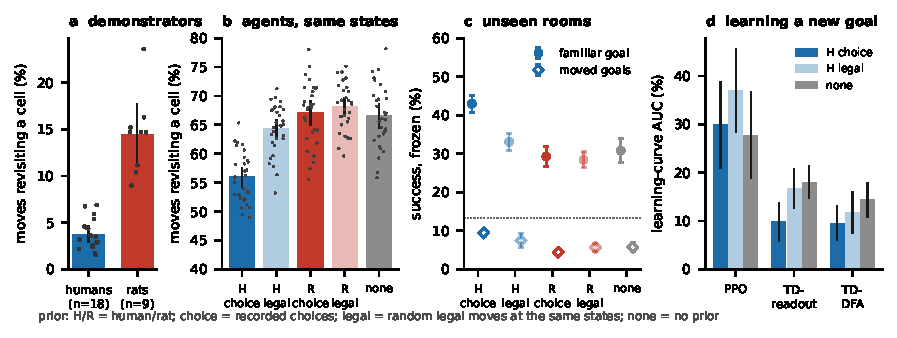
\includegraphics[width=\textwidth]{figs/fig_camera_story.pdf}
\caption{\textbf{The story in one figure.} \textbf{a}~Real demonstrators in the same maze~\cite{decothi2022}: humans
almost never step back onto a cell they have visited; rats do so about four times as often (dots: individuals).
\textbf{b}~Visual agents imitate these choices at the \emph{same} recorded states and then receive identical
reinforcement learning; the legal control keeps the states and replaces the choices by random legal moves. Only
human choices lower the agents' revisiting (dots: seeds, 16 unseen rooms). \textbf{c}~The same frozen agents in
unseen rooms: human choices transfer with the familiar goal; open symbols: moved goals. \textbf{d}~Learning a new
goal with PPO or with local, backpropagation-free three-factor rules. Bars: means; lines: 95\% CIs.}
\label{fig:teaser}
\end{figure*}

\begin{figure*}[t]
\centering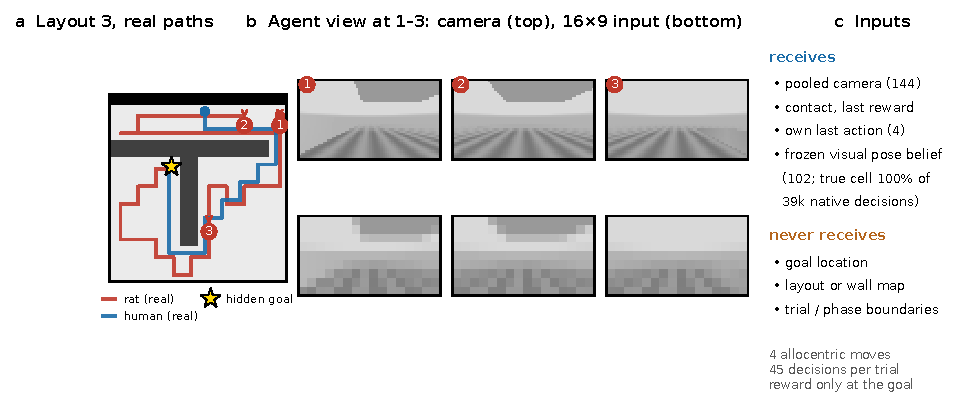
\includegraphics[width=\textwidth]{figs/fig_task.pdf}
\caption{\textbf{The task.} \textbf{a}~One of the seven source layouts with a real rat and human
path~\cite{decothi2022}. \textbf{b}~What the agent receives: a 64$\times$36 render with fog that hides all but
adjacent modules (top) and the 16$\times$9 pooled input (bottom). \textbf{c}~The input contract. The pose belief
(Sec.~\ref{sec:belief}) is computed from the agent's own views with an open-arena template; no wall map is used.}
\label{fig:task}
\end{figure*}


\section{Introduction}
A demonstration shows an agent both \emph{where} to go (visited states) and \emph{what} to do there (choices).
Behaviour-cloning (BC) priors from humans and animals help reinforcement learning~\cite{sreeramdass2025gsd,jia2024d3il,wan2025qdirl,zador2023},
but the usual baselines (no prior, shuffled labels) change state coverage too. We hold coverage fixed: at the exact
recorded states of rats and humans in the cross-species maze of de Cothi et al.~\cite{decothi2022}, we replace the
recorded choices by random \emph{legal} moves (pipeline figure in the supplement) and ask whether the choices make visual
agents~\cite{mirowski2017,banino2018,crosby2020animalai} navigate better in rooms they have never seen.
The answer follows one thread (Fig.~\ref{fig:teaser}): humans rarely revisit a cell (\NatHum\% of moves; rats
\NatRat\%), agents that imitate human choices inherit this and loop less, and this is what transfers to unseen rooms.
The human advantage is claimed for frozen agents with the familiar goal only; moved goals and continued learning
are tested separately.
We then follow the choices through three questions, each with its own test and bound: how far they carry out of
distribution (unseen layouts, moved goals, continued learning), what they do to forgetting when a second goal is
learnt, and where their content lives in vision--language--action geometry (views, captions, actions, networks and
predicted cortex).

\noindent\textbf{Contributions.}
(1)~The legal-uniform label control.
(2)~A causal first-person reconstruction of the maze with a characterised input contract (Fig.~\ref{fig:task}).
(3)~Registered, paired-seed evidence that human choices improve frozen same-goal transfer, confirmed in fresh
rooms, camera-only and against stronger teachers (Table~\ref{tab:main}, Figs.~\ref{fig:teaser}--\ref{fig:ladder}).
(4)~Moved-goal tests, frozen and with learning by PPO or by local three-factor rules without backpropagation,
plus loop, belief and evaluation diagnostics (Figs.~\ref{fig:showcase}--\ref{fig:learning}).
(5)~Forgetting with PPO, local rules and brain-constrained circuits, and the vision--language--action geometry of
views, captions, actions, networks and predicted cortex (Figs.~\ref{fig:viewroute}--\ref{fig:kpi}).
The full sequential-learning, predicted-cortex and alignment studies, including the untrained representation and
closed-loop controls, are in the supplement.

\section{Benchmark and agents}
\textbf{Task.} Rats (physical maze) and humans (head-mounted VR) navigated a 10$\times$10 grid of identical modules
to a hidden goal at (3,3); modules changed between layouts, fog limited sight to adjacent modules, and a curtain was
the only distal cue~\cite{decothi2022}. We re-render each recorded state as a first-person view (Fig.~\ref{fig:task});
the agent moves in four directions, feels contact, is rewarded at the goal, and has 45 decisions per trial.

\textbf{Pose belief.}\label{sec:belief} A frozen grid Bayes filter~\cite{fox1999} matches each view to an
\emph{open-arena} template atlas (400 views, no internal walls) and shifts its posterior by each move unless contact
is felt. It never receives the wall map, goal or true position. It is near exact in clean rooms (top-1 \Bclean) and
fails under dimming (\Bdim; Fig.~\ref{fig:diag}d). Camera-only refits remove it.

\textbf{Agents.} One 64$\times$64 feed-forward actor--critic (no memory; 252 inputs: pooled pixels, contact,
reward, last action, belief) for every arm. Priors imitate 6,000 recorded moves per species (layouts 1--5, 20 epochs):
\begin{equation}
\mathcal L_c(\theta)=-\tfrac{1}{3N}\textstyle\sum_{i,j}\log\pi_\theta(y_i^c\mid o_{ij}),\quad
y_i^{\rm real}=a_i,\; y_i^{\rm legal}\sim\mathcal U(\mathcal A_{\rm legal}(x_i)),
\label{eq:bc}
\end{equation}
over three textures $j$; \emph{sham} shuffles rat labels within subject and layout, \emph{cold} skips imitation.
All arms then get the same 524,288 PPO~\cite{schulman2017ppo} interactions.

\textbf{Evaluation.} Frozen probes \emph{sample} actions (seeded): 16 rooms $\times$ 10 starts $\times$ 3 textures.
The paired contrast $\widehat\Delta=\frac1n\sum_s\frac{1}{|\mathcal R|}\sum_u(p^{\rm real}_{s,u}-p^{\rm legal}_{s,u})$
is in percentage points (pp), with paired $t$-intervals and Holm correction within registered families. A trial is
\emph{trapped} if it times out within $\leq$4 cells over its last 16 decisions. Seeds measure training variability,
not biological replication.

\begin{table*}[t]
\centering\small\setlength{\tabcolsep}{3pt}
\begin{tabular}{@{}lccc@{}}
\toprule
Test (frozen unless noted) & human $-$ legal & human $-$ scratch & rat $-$ legal\\
\midrule
Familiar goal, 16 rooms & 10.1 {\scriptsize[7.2,13.0]} & 12.0 {\scriptsize[8.4,15.6]} & 0.6 {\scriptsize[$-$2.4,3.5]}\\
Familiar goal, 16 fresh rooms$^{\rm R}$ & 9.9 {\scriptsize[6.9,12.9]} & 12.2 {\scriptsize[8.7,15.7]} & 0.9 {\scriptsize[$-$2.7,4.4]}\\
\quad camera only (10 seeds) & 15.2 {\scriptsize[5.9,24.5]} & 22.3 {\scriptsize[16.1,28.4]} & --\\
Moved goals, fresh rooms$^{\rm R}$ & \PMvLegal\ {\scriptsize[\PMvLegallo,\PMvLegalhi]} & \PMvScratch\ {\scriptsize[\PMvScratchlo,\PMvScratchhi]} & \PMvRat\ {\scriptsize[\PMvRatlo,\PMvRathi]}\\
\quad camera only, predicted mouse cortex$^{\rm c}$ & 3.7 {\scriptsize[$-$3.1,10.6]} & 4.3 {\scriptsize[$-$4.0,12.6]} & --\\
\quad camera only, random-core control$^{\rm c}$ & 0.7 {\scriptsize[$-$4.6,6.0]} & 6.1 {\scriptsize[1.6,10.6]} & --\\
Human $-$ rat, fresh rooms: real / legal labels & \multicolumn{3}{c}{13.7 {\scriptsize[10.3,17.1]} \;/\; 4.7 {\scriptsize[1.9,7.4]}}\\
E1: online PPO, layouts 6--7 & 7.7 {\scriptsize[$-$3.8,19.3]} & -- & 5.1 {\scriptsize[$-$5.6,15.9]}\\
\bottomrule
\end{tabular}
\caption{\textbf{Main contrasts} in pp (paired seeds, 30 unless noted; unadjusted 95\% CIs). R: registered before
its own outcome. c: 10 seeds, original 16 rooms, pixels replaced by predicted mouse visual-cortex responses
(Sec.~\ref{sec:brain}). Learning a moved goal: Fig.~\ref{fig:learning}.}
\label{tab:main}
\end{table*}

\section{Results}
\subsection{Out-of-distribution transfer: same states, familiar goal}
\label{sec:ood}
\begin{figure*}[t]
\centering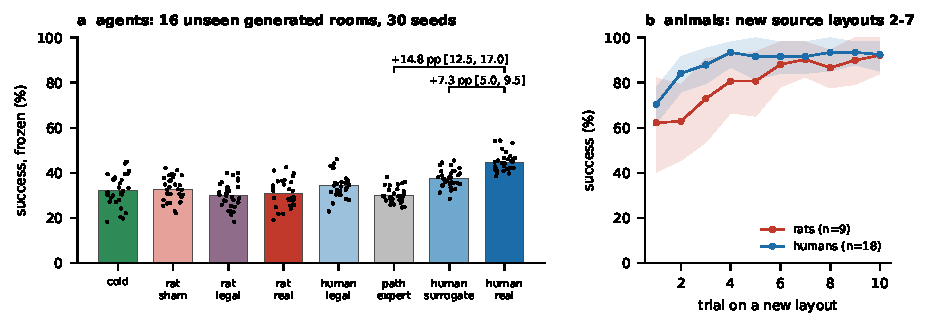
\includegraphics[width=\textwidth]{figs/fig_ood_pp.pdf}
\caption{\textbf{Frozen agents in 16 unseen rooms, familiar goal (3,3).} \textbf{a}~Success per arm (dots: seeds);
path expert and surrogate relabel the same human states. \textbf{b}~Real animals on new layouts: a descriptive
reference, not a matched comparison. Shading: 95\% bootstrap CI over subjects.}
\label{fig:ood}
\end{figure*}

\textbf{Human choices transfer; rat choices do not.} Human-choice agents succeed in 44\% of trials, legal-label
agents in 34\% and scratch in 32\% (Fig.~\ref{fig:ood}); the 10 pp gain replicates in 16 fresh rooms registered
before any outcome (positive in all 16 rooms), in camera-only refits, and against shortest-path, entropy-matched and
goal-bias teachers on the same states (Table~\ref{tab:main}, Fig.~\ref{fig:e2controls}). Rat choices match legal
labels. Compared directly, human-choice agents beat rat-choice agents by 13.7 pp ($[10.3,17.1]$, fresh rooms);
with legal labels at each species' own states the gap is 4.7 pp ($[1.9,7.4]$). About a third of the species gap is
\emph{where} each species went and two thirds is \emph{what it chose} (interaction 9.0 pp, $[4.5,13.6]$; the identity
and the coverage match of the legal control are machine-checked in Lean, supplement). Species and
apparatus coincide, so this is a dataset contrast.

\begin{figure}[t]
\centering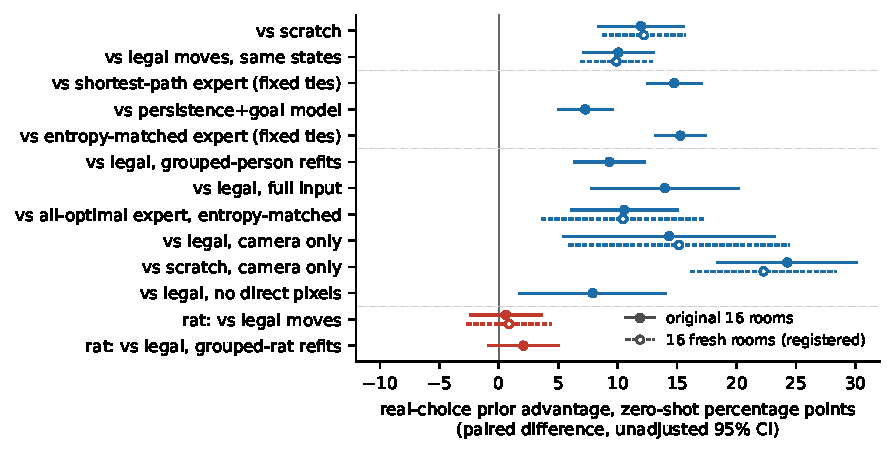
\includegraphics[width=\linewidth]{figs/fig_e2_controls_pp.pdf}
\caption{\textbf{Every control on the same states} (frozen, familiar goal). Real-choice prior minus comparison,
pp, unadjusted 95\% CIs. Filled: original rooms; open: fresh rooms registered before any outcome.}
\label{fig:e2controls}
\end{figure}

\textbf{Robust to geometry, noise, texture and capacity; dimming breaks the belief} (Fig.~\ref{fig:ladder}).
Under $\times0.75$ dimming all arms fall to 13--21\% because the belief fails (Fig.~\ref{fig:diag}d); camera-only
agents trained with brightness augmentation recover the gain (16.3 pp). Replacing human goal-progress labels with
matched non-progress moves costs 23.7 pp (supplement).

\begin{figure}[t]
\centering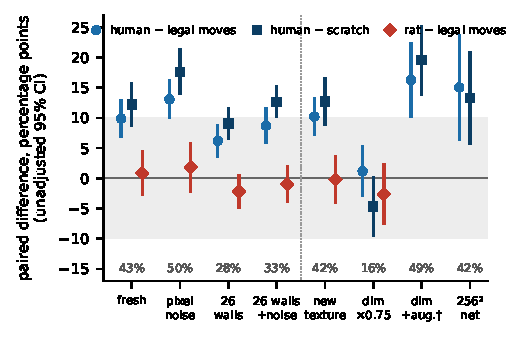
\includegraphics[width=\linewidth]{figs/fig_e2_ladder_pp.pdf}
\caption{\textbf{Robustness} (registered; 16 rooms each). Fresh, pixel-noise and 26-wall rooms; a further room set
with new textures or dimming; a 256$\times$256 network; $\dagger$ camera-only with brightness augmentation.
Numbers: human-choice success.}
\label{fig:ladder}
\end{figure}

\subsection{Where transfer stops: moved goals, loops and evaluation policy}
\label{sec:moved}
\begin{figure*}[t]
\centering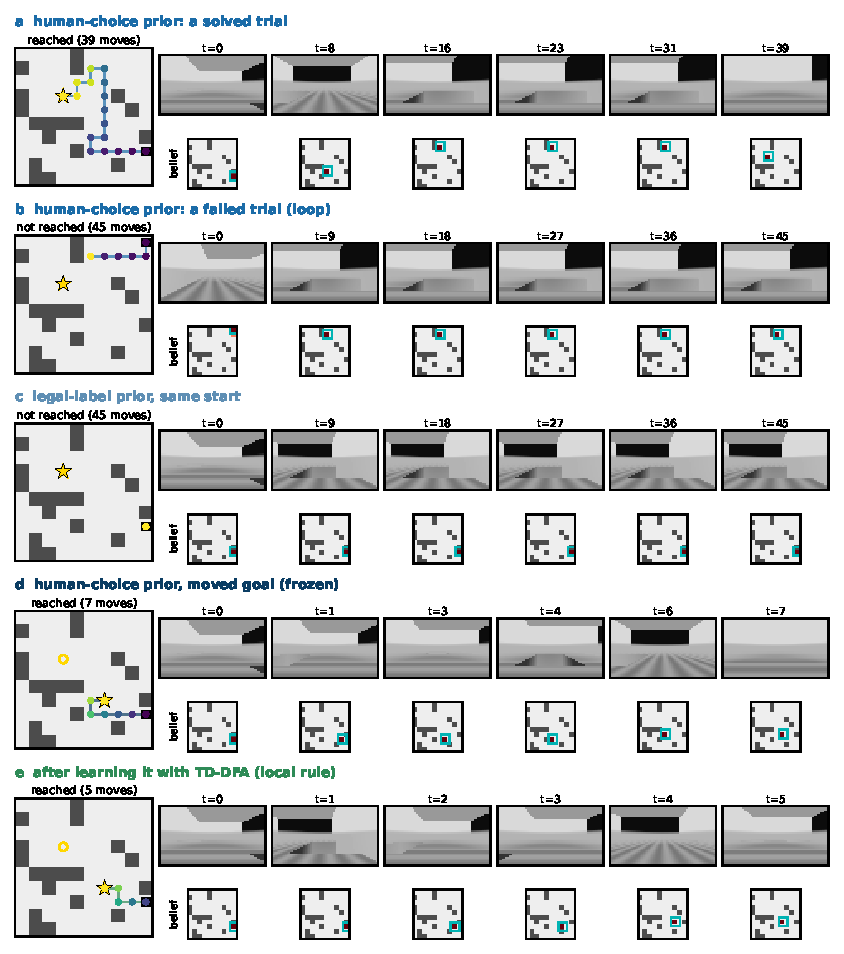
\includegraphics[width=\textwidth]{figs/fig_camera_showcase.pdf}
\caption{\textbf{What the agents see, believe and do} (fresh room, seed 1000; trials chosen by rule, not by outcome:
\textbf{a}~the human-choice agent's first solved trial of $\geq$10 moves, \textbf{b}~its first failed trial,
\textbf{c--e}~the start and texture of \textbf{a}). Left: path (dark$\to$light = early$\to$late), star: goal,
circle: familiar goal. Top strip: the agent's first-person view; bottom: its pose belief (red) and true cell (cyan).
Failures are loops: \textbf{b} and \textbf{c} stay at a wall for most of the trial.}
\label{fig:showcase}
\end{figure*}
\begin{figure*}[t]
\centering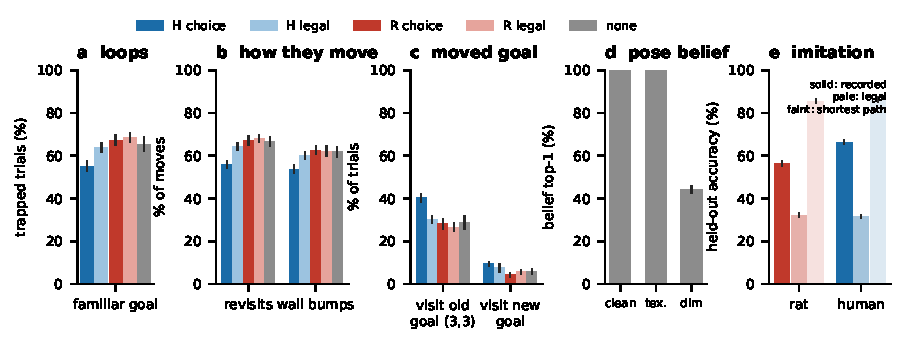
\includegraphics[width=\textwidth]{figs/fig_camera_diag.pdf}
\caption{\textbf{How the agents move} (frozen, 16 fresh rooms, 30 seeds). \textbf{a}~Trapped trials.
\textbf{b}~Moves that revisit a cell or bump a wall. \textbf{c}~With a moved goal: trials that enter the old goal
(3,3) and the new goal. \textbf{d}~Pose-belief top-1 accuracy. \textbf{e}~Held-out imitation accuracy, recorded
versus legal labels (and shortest path). Bars: means; lines: 95\% CIs.}
\label{fig:diag}
\end{figure*}

\textbf{Moved goals.} All training used goal (3,3), so a frozen agent might only remember where the goal is. We
registered three moved goals per fresh room (mirrors of (3,3)) before any outcome. \MGresults

\textbf{Loops: what the human choices teach.} \Ftrap\ of failed trials are loops (Fig.~\ref{fig:showcase}b,c).
Human-choice agents revisit \HLrevisit\ pp fewer cells and are trapped in \HLtrap\ pp fewer trials
(Fig.~\ref{fig:diag}b). Across seeds, each point of trapping costs \LoopSlope\ pp of success; at equal trapping the
human gain shrinks to \LoopInt\ pp ($[\LoopIntlo,\LoopInthi]$, post hoc). Most of the transferable content is thus the
humans' own habit of not going back (Fig.~\ref{fig:teaser}a), which a memoryless agent cannot infer from coverage. Pixel noise also breaks loops (trapped
\CleanTrapH\%$\to$\NoiseTrapH\% for human choices, \CleanTrapL\%$\to$\NoiseTrapL\% for legal labels), which is why it
raises every arm's success.

\textbf{Evaluation policy.} Probes sample actions, as registered; greedy actions lower every arm because a
deterministic memoryless system that repeats a state never reaches the goal (Lean~4 proof; supplement). \GRresults

\textbf{Rat choices are learnable, but less predictable.} Held-out imitation accuracy is \BCrat\ (rat) and
\BChuman\ (human) versus \BClegalrat\ and \BClegalhuman\ for legal labels (Fig.~\ref{fig:diag}e): rat choices carry
about half the predictable information (\BCinforat\ versus \BCinfohuman\ nats per move). The rat null holds only
for these reconstructed inputs.

\subsection{Learning a moved goal: PPO and local learning rules}
\label{sec:learning}
\begin{figure*}[t]
\centering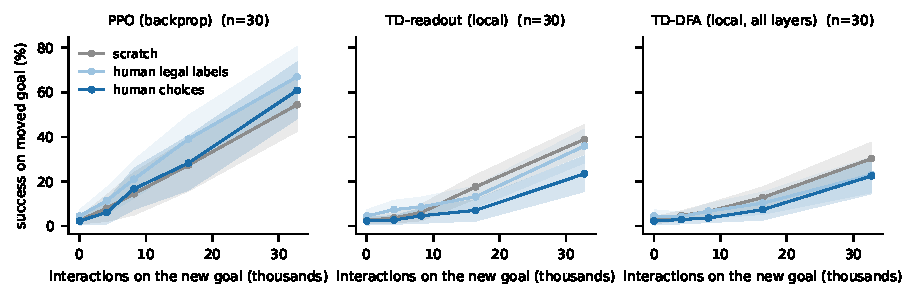
\includegraphics[width=\textwidth]{figs/fig_camera_learning.pdf}
\caption{\textbf{Learning a moved goal, three learning rules, three priors} (30 seeds; one fresh room each; frozen
30-trial probes; bands: 95\% CIs). TD-readout and TD-DFA: TD error $\times$ local eligibility trace only (no
backpropagation, no replay); TD-DFA sends hidden credit through fixed random feedback.}
\label{fig:learning}
\end{figure*}
Each frozen checkpoint learns a moved goal for 32,768 interactions with one of three rules from the same weights:
PPO; \emph{TD-readout}, an online TD($\lambda$) actor--critic on the output synapses in which the TD error gates a
local eligibility trace, a three-factor rule~\cite{sutton2018rl,fremaux2013actorcritic,fremaux2016neuromodulated};
(its local update is exactly the policy gradient of the output synapses, proven in Lean with Mathlib; supplement)
and \emph{TD-DFA}, the same rule in every layer with hidden credit from fixed random feedback (direct feedback
alignment~\cite{nokland2016dfa,lillicrap2016fa}, as in random-feedback e-prop~\cite{bellec2020}). As in e-prop,
each synapse scales its own update with Adam statistics; there is no backpropagation, replay or batch reuse. Local
rates were set on separate rooms and seeds; a first version with fixed-rate updates failed calibration and was
replaced before testing (supplement). We then searched the plasticity architecture (which layers learn; random
feedback or the modulo error routing of Error Diffusion~\cite{yamada2026ed}) jointly with the rule's settings
(Optuna TPE~\cite{akiba2019optuna}, dev rooms only; the same search tunes living neuron cultures that navigate grids~\cite{zhou2026embodied}) and tested the best configurations once on the 30-seed protocol. \LRresults

\subsection{Vision--language--action geometry: the move is in the view, the route in the choice}
\label{sec:brain}
\begin{figure}[t]
\centering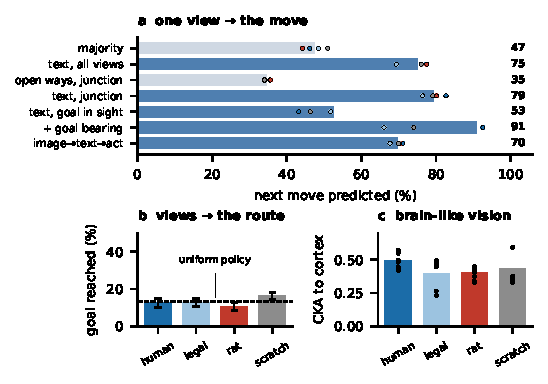
\includegraphics[width=\linewidth]{figs/fig_view_route.pdf}
\caption{\textbf{A view holds the move, not the route.} \textbf{a}~Next move predicted from one view in held-out rooms
(captions without action words; bars: mean or pooled rows; dots: policy arms). \textbf{b}~Agents driven by the
image$\to$text$\to$action map, 30 trials per room (95\% CIs). \textbf{c}~Hidden-layer CKA to the predicted mouse
cortex (all 9,941 units; dots: seeds; shuffled $\le$0.01).}
\label{fig:viewroute}
\end{figure}
The human advantage is a habit of not going back (Sec.~\ref{sec:moved}). Can it be read from what the agent
sees~\cite{schnaus2026rosetta,huh2024platonic}? One view gives the move: text describing only the view predicts it
(75\% versus 47\% majority; 91\% once the goal is in sight with its bearing), and image$\to$text$\to$action maps fitted on
other seeds recover it (70\%; Fig.~\ref{fig:viewroute}a). Views do not give the route: agents driven by these moves
reach the goal at the uniform rate (b, versus 32--45\% with their own heads), and without known pairs the authors'
aligner cannot match views to actions (FOSCTTM 0.47--0.55; chance 0.5), yet it aligns networks trained on the same choices (0.06 across seeds; 0.50--0.59 versus rat or scratch). Same views, different choices; human choices
supply the route. With pixels replaced by the mouse visual-cortex responses a foundation model~\cite{wang2025fnn}
predicts for the agent's frames, human choices keep their direction (revisits $-3.0$ pp, $[-7.0,0.9]$; 10 seeds), and
human-choice networks are the closest to this cortex (c; identical on 144 PCs; supplement).

\subsection{Forgetting and generalisation of new learning}
\label{sec:kpi}
\begin{figure*}[t]
\centering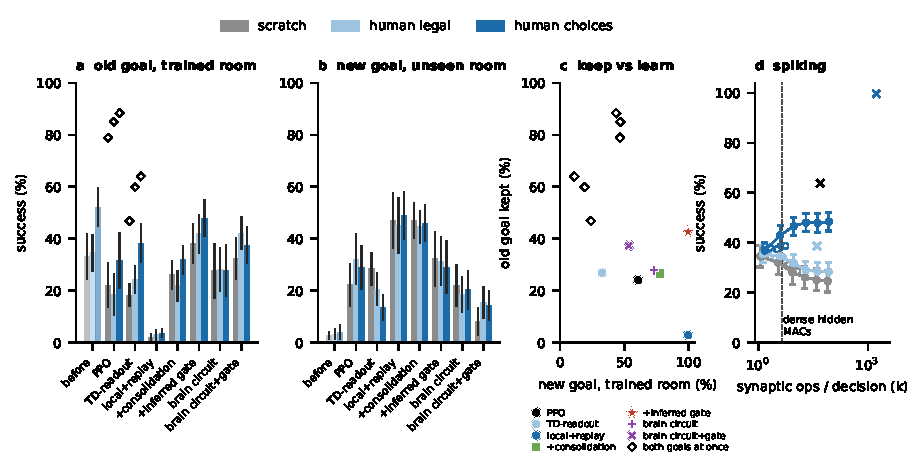
\includegraphics[width=\textwidth]{figs/fig_camera_kpi.pdf}
\caption{\textbf{The four claims, measured on this task} (30 seeds per bar; 95\% CIs). After each agent learns the
moved goal in one room, frozen probes test \textbf{a}~the old goal in that room (forgetting) and \textbf{b}~the new goal in
the paired room it never trained in (generalisation). Pale bars: before learning. Learners: PPO; TD-readout; local rules with
replay and a sparse expansion; plus consolidation and old replay; plus an inferred context gate; a mushroom-body-like circuit with awake replay, without and with the gate.
\textbf{c}~Learner means, old goal kept versus new goal learnt; diamonds: both goals at once. \textbf{d}~Integrate-and-fire
conversion: success versus synaptic operations per decision (operation counts, not energy); filled: fixed $T=1$--$32$;
open: stop at a confidence bound; crosses: learned networks at $T=16$; dashed: the dense prior's hidden multiply-accumulates.}
\label{fig:kpi}
\end{figure*}
The submitted version named continual learning, forgetting, generalisation and spiking efficiency as motivations
without measuring them for the learners. We now measure all four on the same agents and rooms (Fig.~\ref{fig:kpi}).
\KPIresults

\FloatBarrier
\section{Discussion and limitations}
At the same states, human choices make frozen visual agents better navigators in unseen rooms with the familiar
goal, partly by looping less. \MGdiscussion\ The same fact explains forgetting and geometry: views hold the move but not the route, so two goals
in the same views collide unless a context signal separates them. A random-legal-label control costs one extra run and should accompany any demonstration prior.
\textbf{Limitations.} Rats (physical maze) and humans (VR) differ in species, apparatus and coverage: a dataset
contrast. Views are reconstructed without touch or smell; the belief is near exact and fails under dimming; the
policy is small, memoryless and below the animals ($\approx$92\% within ten trials, Fig.~\ref{fig:ood}b). Local
learners start from a backpropagation-trained network. Follow-ups added after earlier results are marked and were
registered before their own outcomes.

\noindent\textbf{Reviewer questions.} Every question raised in review is answered, with pointers, in supplement
Sec.~Q\&A.

\noindent\textbf{Implementation assistance.} Claude Code and Codex assisted coding and figures (supplement).

{\small
\bibliographystyle{ieeenat_fullname}
\bibliography{v4n_refs}
}
\end{document}
